\documentclass[12pt]{article}

\usepackage{graphicx}
\graphicspath{ {../plots/} }
\usepackage{caption}
\usepackage{subfigure}

\title{Traffic Accidents Analysis}
\date{}

\begin{document}

\maketitle

% INTRODUCTION
% Introduce the project
% What is the data
% What is the goal
% How is the analysis structured?

% ANALYSIS

% EDA

Upon first inspection of the data, it was determined that there exist two primary SPIKES in accident frequency within the ranges 8am-10am, and then again from 3pm 7pm Figure \ref{time_of_day}. These are the times of commute, and so such increases are to be expected.

\begin{figure}[h]
\centering     %%% not \center
\subfigure[Accidents by time of day.]{\label{fig:a}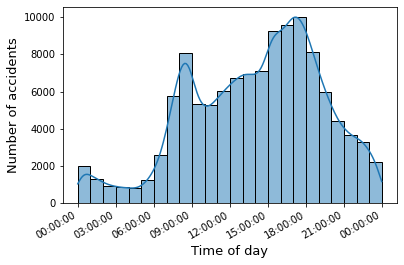
\includegraphics[width=0.45\textwidth]{time_of_day}}
\subfigure[Accidents by day of the week.]{\label{fig:b}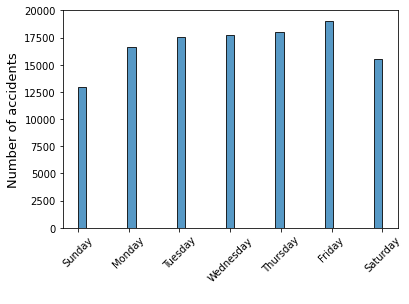
\includegraphics[width=0.45\textwidth]{day_of_week}}
\caption{Number of accidents.}
\end{figure}

% Hypotheses

% PREDICTIONS

% RECOMMENDATIONS

\end{document}